%
% 2
%
\section{\system}
\label{repiano}

{\system}は、
自分の過去の演奏履歴を活用することによって
ひとりでも楽しく演奏を行なうことを可能にするシステムである。
演奏中に以下のボタンを押すことで楽しい演奏ライフをサポートする。

%2.1
\subsection{録音再生ボタン}
\label{recplaybutton}

直前の無音部分から現在までの演奏を登録して、繰り返し再生を行う。\figref{recplay1}
録音開始の操作は不要で、演奏の途中や、
演奏が終わってから登録可能な点が既存のツールとは異なる大きな特徴である。
登録部分の中に演奏の繰り返しが含まれる場合はDynamic Macro\cite{masui}を適用し、
繰り返し部分だけを登録して連続再生を行う。
また、再生中に重ねて演奏を行なうことができ、そこで録音再生ボタンを押すとその演奏も新たに登録される。
この演奏は最初に登録された繰り返しフレーズのタイミングに合わせて記録されるため、
時間が経過してもずれることなく再生され続ける。

\begin{figure}[tb]
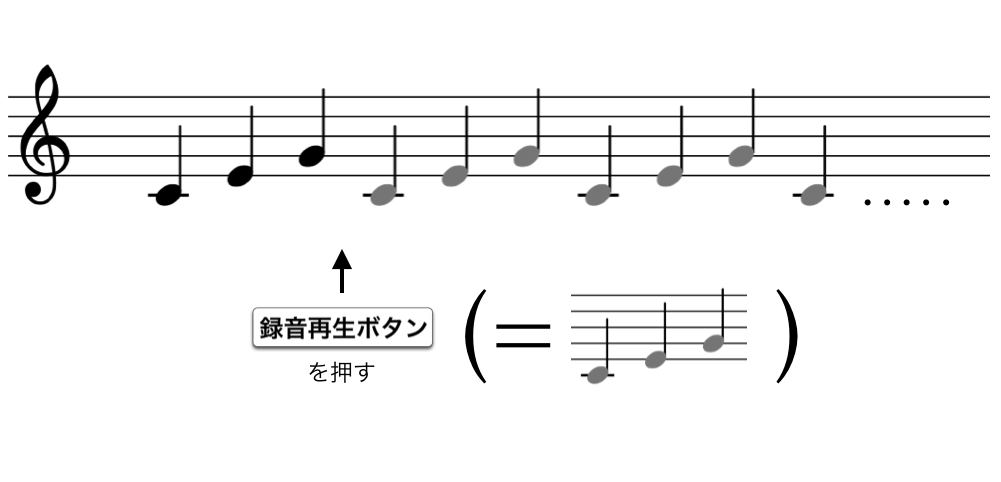
\includegraphics[width=8cm,bb=0 0 1054 481]{images/rp1.png}
\centering
\caption{演奏の登録}
\label{recplay1}
\end{figure}

%2.2
\subsection{やり直しボタン}

\ref{recplaybutton}で重ねていった演奏を、新しいものから順に取り消す。
登録された演奏はそれぞれ独立して管理されているので、
やり直しボタンによってすぐ以前の状態に戻すことができる。
